% !TEX root = classicthesis.tex

%************************************************
\chapter{A Bytecode Implementation}\label{ch:bytecode} % $\mathbb{ZNR}$
%************************************************

\section{Why not AST?}

We choose a bytecode implementation for it's speed compared to the main rival candidate for an interpreter; a tree-walk interpreter. We've explained the general reason for this in our design overview. 

In more depth, when we write any piece of code that's to be compiled using an AST, it's just not memory efficient. Each fragment of code becomes an AST node. Take the expression \verb%1 + 2% turns into a flurry of objects with pointers, each adding an extra 32 or 64 bits of overhead to the object. Not only this, when spreading our data across the heap in a loosely connected web of objects, we have problems with spatial locality. 

Spatial locality (also known as data locality) refers to the use of data elements within relatively close storage locations. Modern CPUs can process data much faster than they can retreive it from RAM, leading to the use of (multiple layers of) caching. If a piece of memory it needs is already in the cache, it can be loaded more quickly, even upto two orders of magnitude faster. 

The CPU ``predicts'' what data we need by pulling in adjacent bytes to what is currently being read from RAM and stores them in cache. If our program next requests some data close enough to be inside that cache line, we end up with a faster program experience. To take advantage of this, the way we represent code in memory should be dense and ordered like it’s read. 

However, when using an AST, the sub-objects can be stored anyway. Every step the tree-walker takes where it follows a reference to a child node may step outside the bounds of the cache and force the CPU to stall until the next data can be recalled from RAM\@. Just the overhead of the tree nodes with all of their pointer fields and object headers tends to push objects away from each other and out of the cache.

\section{Why Bytecode?}

Let's consider the other end of the speed spectrum first, compiling to native machine code. Compiling directly to the native instruction set the chip supports is what the fastest languages do, where the CPU cranks through the instructions, decoding and executing each one in order. There is no tree structure like our AST, and control flow is handled by jumping from one point in the code directly to another. This comes at a cost, as firstly this comilation process is not easy, especially with newer chips which more complicated architectures. Furthermore, there is no portability, as we'd only be producing for one architecture type of the multiple that are used today. To get our language on all of them, we'd need to learn all of their instruction sets and write a separate back end for each one.

Bytecode is in the middle of both extremes of these implementations, retaining the portability of a tree-walker and sacrifices some simplicity for an increase in performance. Although bytecode resembles machine code in it's dense, linear sequence of binary instructions, simpler, higher-level instruction set than any real chip. This keeps the overhead low, and takes advantage of the caching feature of a chip. 

It's essentially like writing for an idealised fantasy instruction set for some perfect architecture. However, obviously when we develop for such an architecture that doesn't exist, we can't actually run it normally. This means we need to write an emulator – a simulated chip written in software that interprets the bytecode one instruction at a time and simulates what the perfect architecture would do. This is known as a \ac{VM}.

This does add overhead, which is why using a bytecode implementation is not as fast as writing native machine code, but in return we receive portability to run on basically any hardware we want. Below we outline our implementation process, although we probably won't build each phase in order.


\begin{figure}[h]
\centering
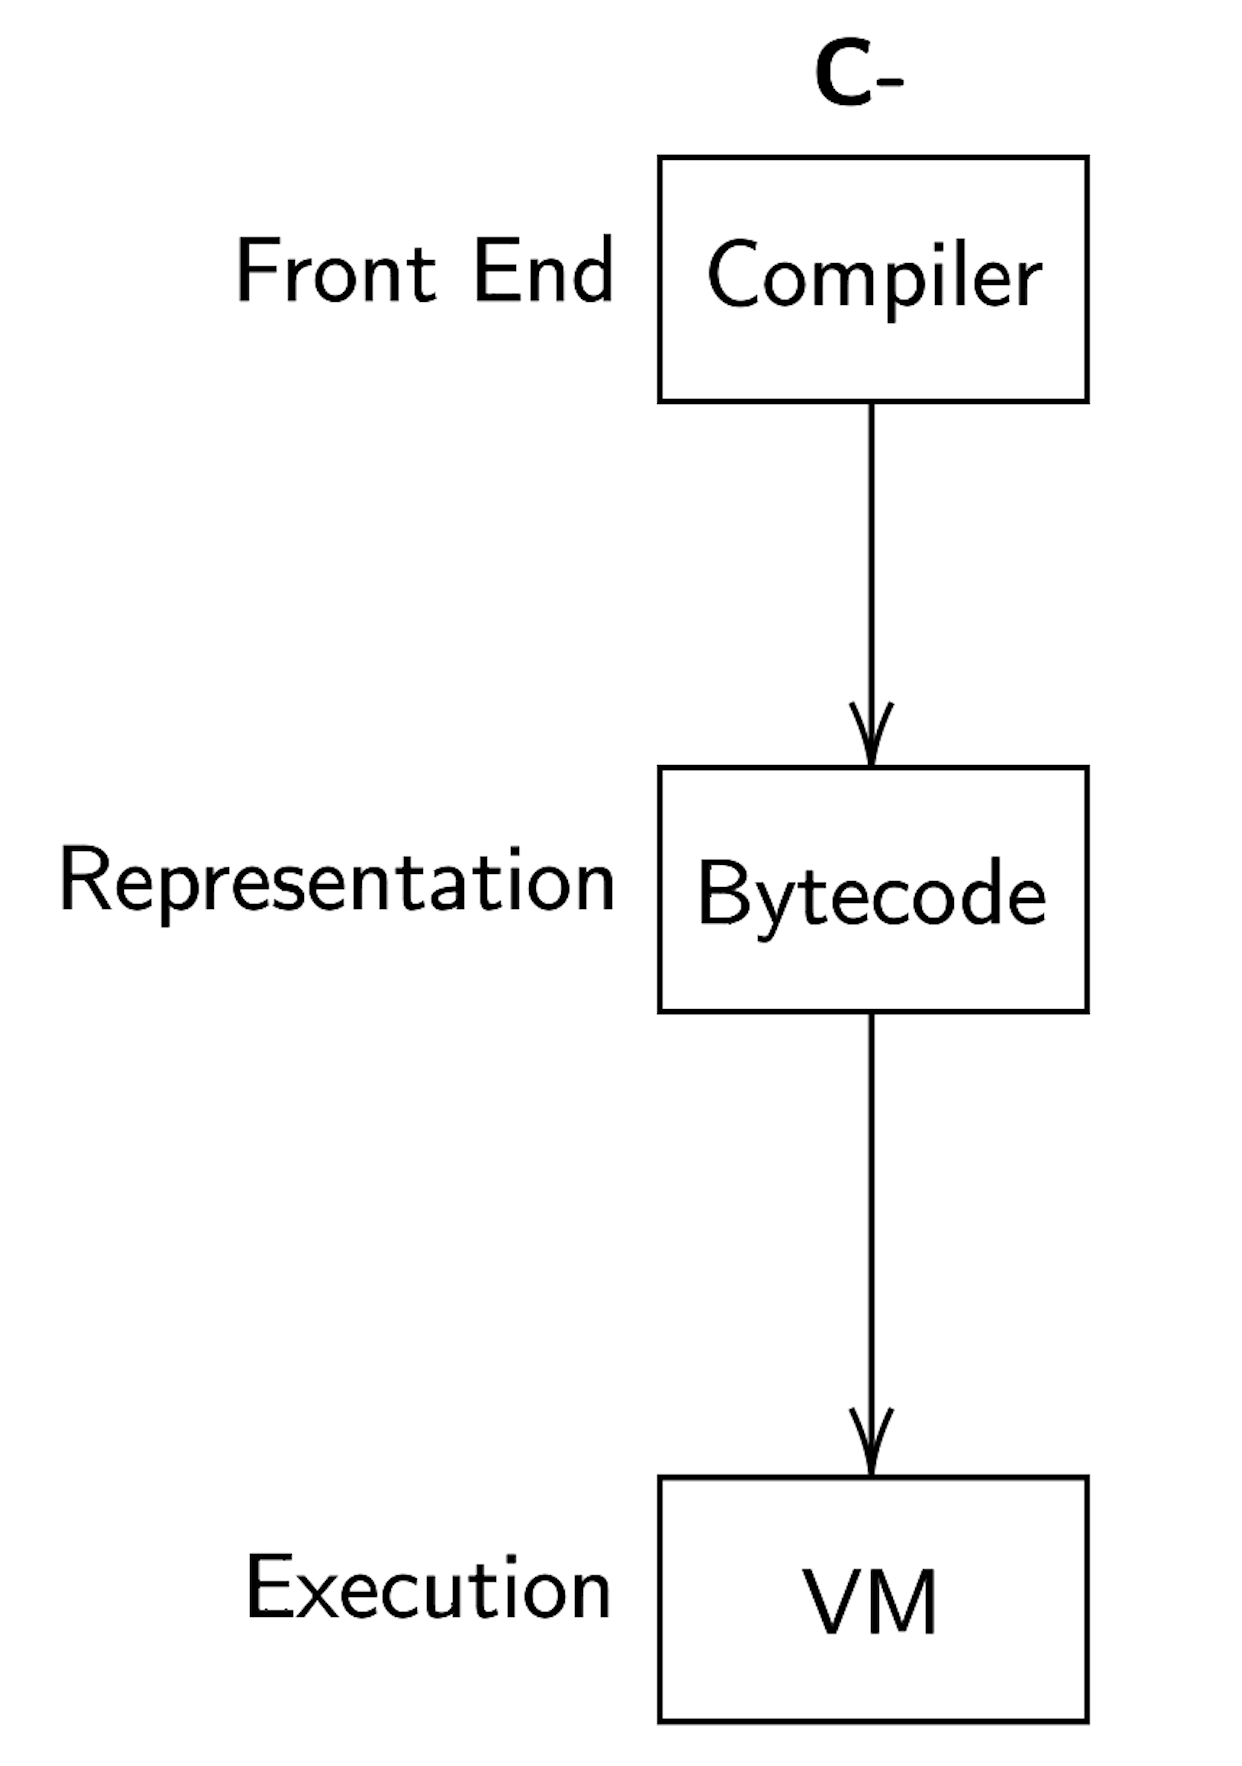
\includegraphics[width=0.35\textwidth]{gfx/process.png}
\caption{Implementation Process}
\end{figure}

\section{Laying the Foundation}

We'll start with our \verb+main()+ function in \verb+main.c+. For now we'll just create an empty function.

\begin{lstlisting}[language=C]
// main.c

#include "common.h"

int main(int argc, const char* argv[]) {
  return 0;
}
\end{lstlisting}

As we can see by the quotation marks, the \verb+common.h+ file is not part of the C standard library. Let's create it now:

\begin{lstlisting}[language=C]
// common.h

#ifndef common_h
#define common_h

#include <stdbool.h>
#include <stddef.h>
#include <stdint.h>

#endif
\end{lstlisting}

This is where we store the additional C types we'll use throughout the process. For now, we've added \verb+NULL+, the C99 \verb+bool+ data type which macros true and false expand to \verb.1. and \verb.0. respectively, and some more specific types of integers such as \verb+uint8_t+ (unsigned integers). 

In \emph{Crafting Interpreters}, Bob Nystrom refers to chunks as sequences of bytecode, so we draw from that to create the module \verb+chunk.h+. In bytecode, each instruction has a one-byte opcode (operation code), which controls what kind of instruction we're dealing with. We define that here. 

\begin{lstlisting}[language=C]
// chunk.h

#ifndef chunk_h
#define chunk_h

#include "common.h"

typedef enum {
  OP_RETURN,
} OpCode;

#endif
\end{lstlisting}

The only instruction \verb+OP_RETURN+, will eventually mean ``return from the currrent function'', but has no use at the moment. 


\subsection{Dynamic Arrays}

Let's now create the \verb+struct+ to hold the data that will be stored alongside the instructions.

\begin{lstlisting}[language=C]
// chunk.h

typedef struct {
  uint8_t* code;
} Chunk;
\end{lstlisting}

This just creates a wrapper arround an area of bytes, however because we don't know how big the array of data needs to be before compiling a chunk we need, it needs to be dynamic. Implementing this is simple, we just need to declare an additional two quantities: the number of elements in the array we have allocated (\verb+capacity+) and how many of these are in use (\verb+count+).

\begin{lstlisting}[language=C]
// chunk.h

typedef struct {
  int count;
  int capacity;
  uint8_t* code;
} Chunk;
\end{lstlisting}

If \verb+count+ is less than \verb.capacity. then adding an element is as simple as allocating the new element to the free space and incrementing count. If there is no spare capacity then our process is as follows: 

\begin{itemize}
 \item Allocate a new array with more capacity and carry over the existing elements from the old array to the new one. 
 \item Store the new capacity and delete the old array
 \item Update \verb+code+ to point to the new array and store the element in the new array
 \item Increment \verb+count+
\end{itemize}

Note that through the use of amortized analysis, we can see that as long as we grow the array by a multiple of its current size, when we average out the cost of a sequence of appends, each append only takes \(\mathcal{O}(1)\).

Now that our \verb.struct. is ready, we can implement the functions to work with it. Because C doesn't have constructors, we need to declare a function to initialize a new chunk.

\begin{lstlisting}[language=C]
// chunk.h

void initChunk(Chunk* chunk);
\end{lstlisting}

Let's implement it by creating a new file, \verb+chunk.c+:

\begin{lstlisting}[language=C]
// chunk.c

#include <stdlib.h>

#include "chunk.h"

void initChunk(Chunk* chunk) {
  chunk->count = 0;
  chunk->capacity = 0;
  chunk->code = NULL;
}
\end{lstlisting}

Note that we don't even allocate a raw array to our dynamic array; it starts of completely empty. Let's create a new function to append a byte to the end of a chunk:

\begin{lstlisting}[language=C]
// chunk.c

void writeChunk(Chunk* chunk, uint8_t byte) {
  if (chunk->capacity < chunk->count + 1) {
    int oldCapacity = chunk->capacity;
    chunk->capacity = GROW_CAPACITY(oldCapacity);
    chunk->code = GROW_ARRAY(uint8_t, chunk->code,
        oldCapacity, chunk->capacity);
  }

  chunk->code[chunk->count] = byte;
  chunk->count++;
}\end{lstlisting}

The first thing that we need to do is see if the current array already has the capacity for the new byte, and if it doesn't we grow the array to make room. This will happen every time on the  first write, as we've set the original \verb+capacity+ to \verb.0.. 

To increase the array's size, we first calculate the new capacity and then adjust the array to match it. These lower-level memory operations are now defined in a new module \verb+memory.h+.

\begin{lstlisting}[language=C]
// memory.h

#ifndef memory_h
#define memory_h

#include "common.h"

#define GROW_CAPACITY(capacity) \
    ((capacity) < 8 ? 8 : (capacity) * 2)

#endif
\end{lstlisting}

Since we're using it in the process of chunks, we should also include it in \verb+chunk.c+ using:

\begin{lstlisting}[language=C]
// chunk.c

#include "memory.h"
\end{lstlisting}

This macro calculates a new capacity based on the current capacity, and for optimal performance, it scales relative to the previous size. Typically, we increase it by a factor of two, although 1.5× is another common choice.

We've also accounted for cases where the current capacity is zero. In such instances, we start with eight elements instead of one, reducing unnecessary memory overhead for very small arrays, albeit at the cost of some wasted space. The choice of the number eight was somewhat arbitrary in this context, as most dynamic array implementations have a similar minimum threshold. 

Once the desired capacity is determined, we proceed to create or expand the array to match that size using the \verb+GROW_ARRAY()+ function.

\begin{lstlisting}[language=C]
// memory.h

#define GROW_ARRAY(type, pointer, oldCount, newCount) \
    (type*)reallocate(pointer, sizeof(type) * (oldCount), \
        sizeof(type) * (newCount))

void* reallocate(void* pointer, size_t oldSize, size_t newSize);
\end{lstlisting}

This macro simplifies a function call to \verb.reallocate(). where the primary work is accomplished. It takes care of determining the size of the array's element type and performing the necessary casting to ensure the resulting \verb+void*+ is of the correct type.

The \verb.reallocate(). function serves as the central function for all dynamic memory management within C-. It handles various tasks such as memory allocation, deallocation, and resizing existing allocations. This consolidation of memory operations into a single function becomes crucial later when we introduce a garbage collector responsible for monitoring memory usage.

The two size arguments provided to \verb.reallocate(). dictate the specific operation to be executed:


\begin{table}[h]
{\centering
\begin{tabular}{|c|c|c|}
\hline
\rowcolor[HTML]{EFEFEF} 
\verb.oldSize. & \verb.newSize.              & Operation                  \\ \hline
0              & Non-zero                    & Allocate new block         \\ \hline
Non-zero       & 0                           & Free allocation            \\ \hline
Non-zero       & Smaller than \verb.oldSize. & Shrink existing allocation \\ \hline
Non-zero       & Larger than \verb.oldSize.  & Grow existing allocation   \\ \hline
\end{tabular} \par}
\end{table}

Although this looks like a lot of different cases to consider for, the implementation is quite simple. We'lll add this to a new file \verb,memory.c,

\begin{lstlisting}[language=C]
// memory.c

#include <stdlib.h>

#include "memory.h"

void* reallocate(void* pointer, size_t oldSize, size_t newSize) {
  if (newSize == 0) {
    free(pointer);
    return NULL;
  }

  void* result = realloc(pointer, newSize);
  return result;
}
\end{lstlisting}


%*****************************************
%*****************************************
%*****************************************
%*****************************************
%*****************************************
